\chapter{Stato dell'arte}\label{sec:Stato dell'arte}

L'Image Captioning è il compito di descrivere il contenuto visivo di un'immagine in linguaggio naturale e viene classificato nella letteratura come un problema image-to-sequence, il cui input è un insieme di pixel di un'immagine che viene codificato come uno o più vettori di feature. La rappresentazione ottenuta viene utilizzata da un ulteriore modello che determina una sequenza di parole.

La parte di comprensione dell'immagine è la componente più complessa poiché la descrizione potrebbe contenere qualsiasi aspetto visivo dell'immagine: può menzionare gli oggetti e i loro attributi, può considerare le caratteristiche della scena (per esempio, indoor/outdoor), o verbalizzare come le persone e gli oggetti nella scena interagiscono. Inoltre, la descrizione può anche riferirsi a oggetti che non sono raffigurati (per esempio, può fare riferimento a persone che aspettano un treno, anche quando il treno non è visibile perché non è ancora arrivato) e fornire conoscenze di base che non possono essere derivate direttamente dall'immagine (per esempio, la persona raffigurata è la Monna Lisa).


La comprensione dell'immagine è necessaria, ma non sufficiente per produrre una buona descrizione, in quanto quest'ultima deve essere completa ma concisa (parlare di tutte e solo le cose importanti nell'immagine) e deve essere formalmente corretta, cioè composta da frasi grammaticalmente ben formate. Da un punto di vista del \acrshort{nlp}, generare una tale descrizione è un problema di \acrfull{nlg}, il quale consiste nella trasformazione di una rappresentazione non linguistica in un testo leggibile dall'uomo. Classicamente, la rappresentazione non linguistica è una forma logica, una query o un insieme di numeri. Nella descrizione delle immagini, l'input è una rappresentazione dell'immagine che il modello di \acrshort{nlg} deve trasformare in frasi in linguaggio naturale.

Inoltre, il compito di descrizione può diventare ancora più impegnativo quando si tiene conto che le buone descrizioni sono spesso specifiche per l'utente. Per esempio, un critico d'arte richiederà una descrizione diversa da quella di un bibliotecario o di un giornalista, anche per la stessa immagine.
%L'obiettivo finale di questo task è quello di trovare una pipeline che elaborare un'immagine in ingresso, ne rappresenta il contenuto generando connessioni tra elementi visivi e testuali, infine la rappresentazione viene trasformata in una sequenza di parole che rispetta la fluidità del linguaggio.

\section{Metodi}
La letteratura esistente, in base all'approccio utilizzato, può essere suddivisa in due categorie principali \cite{bernardi2016automatic}: 
\begin{enumerate}
\item\textbf{Direct Generation models};
\item\textbf{Retrieval-based models};
\end{enumerate}
In questa sezione ci soffermeremo maggiormente sulla prima tipologia poiché è quella più utilizzata al giorno d'oggi ed è quella che ha consentito il raggiungimento dei risultati dello stato dell'arte.
\subsection{Direct Generation models}\label{directmodel}
Il task di Image Captioning è stato generalmente affrontato utilizzando questa tipologia di modelli, la quale si basa su pipeline composte da un codificatore visivo (\textbf{visual encoder}) che genera una rappresentazione dell'immagine e questa codifica viene utilizzata come input da un modello linguistico (\textbf{language model}) che si occupa della generazione del testo.
Nel corso degli anni, entrambi i componenti sono evoluti considerevolmente attraverso lo sfruttamento delle regioni delle immagini, attributi visivi, l'introduzione delle multi-modal connections, approcci fully-attentive e strategie di early-fusion tipo \acrshort{bert}. 
%Tuttavia, nonostante i risultati impressionanti, la ricerca sulla didascalia delle immagini non ha ancora raggiunto una risposta definitiva.
Inoltre, i modelli che sono stati sviluppati hanno affrontato questo problema concentrandosi su svariati aspetti poiché le persone hanno diversi stili di descrizione. Infatti, le didascalie delle immagini possono essere percettive, quando si concentrano su attributi visivi di basso livello; non visive, quando riportano informazioni implicite e contestuali; concettuali, quando descrivono l'effettivo contenuto visivo (per esempio entità visive e loro relazioni). Quest'ultimo è comunemente riconosciuto come l'obiettivo dell'Image Captioning, questa definizione comprende descrizioni che si concentrano su aspetti diversi e a vari livelli di dettaglio (per esempio, includendo o meno gli attributi, menzionando entità nominate o concetti di alto livello, descrivendo solo parti salienti o anche dettagli più fini). 

\subsubsection{Visual Encoder}
L'obiettivo di questo componente è quello di fornire una rappresentazione significativa del contenuto visivo dell'immagine e i vari approcci che sono stati utilizzati possono essere suddivisi nelle seguenti categorie \cite{stefanini2021show}: metodi \textbf{non-attentive} che si basano su feature globali estratte tramite una \acrshort{cnn}; metodi \textbf{additive attentive} che rappresentano il contenuto visivo usando griglie; metodi con \textbf{attention over visual regions} che estraggono regioni dall'immagine; metodi basati su grafi (\textbf{graph-based}) che aggiungono relazioni visive tra le regioni dell'immagine; metodi \textbf{self-attentive} che si basano sui Transformer.
\paragraph{Non-Attentive}
Questo è l'approccio più vecchio utilizzato per la codifica visiva dell'immagine ed è effettuata utilizzando l'attivazione di uno degli ultimi strati di una \acrshort{cnn} (escludendo la componente fully-connected). Questa tecnica è molto semplice e fornisce una rappresentazione compressa; tuttavia, le informazioni sono eccessivamente ristrette mancando di granularità, rendendo difficile per un modello di captioning la produzione di descrizioni dettagliate. 
\paragraph{Additive Attentive}
Questo approccio cerca di risolvere le criticità della tecnica precedente fornendo una rappresentazione più ricca di dettagli e per ottenere questo risultato utilizza l'additive attention \cite{bahdanau2014neural, stefanini2021show}.
Questo meccanismo viene utilizzato per connettere gli strati convoluzionali della \acrshort{cnn} con gli stati nascosti del language model. Questa tipologia di attention si basa solitamente su una single-layer \acrshort{ffn} che usa una hyperbolic tangent non-linearity per calcolare i pesi di attenzione, i quali indicano quanto una porzione dell'immagine è importante per la predizione della caption.
Quindi, l'immagine viene trattata come una griglia di elementi ottenuta dall'output di uno strato convoluzionale di una \acrshort{cnn}, gli elementi di questa griglia sono utilizzati per calcolare un peso che specifica l'importanza relativa di quell'elemento per generare la parola successiva.
%Formalmente dati due insiemi di vettori ${x_1, ..., x_n}$ (elementi della griglia) e ${h_1, ..., h_m}$ (stati nascosti del modello linguistico), il punteggio di attenzione additiva tra il vettore $h_i$ e il vettore $x_j$ è calcolato come: 
%\begin{equation}
%	f_{att}(h_i, x_j) = W_3^T \cdot tanh(W_1 \cdot h_i + W_2 \cdot x_j) 
%\end{equation}
%dove $W_1$ e $W_2$ sono matrici di pesi, mentre $W_3$ è un vettore di pesi per effettuare una combinazione lineare. Infine, viene applicata una funzione di softmax per ottenere una distribuzione di probabilità p($x_j|h_i$) che specifica la rilevanza della codifica di $x_j$ per $h_i$.

\paragraph{Attention Over Visual Regions}
%Questa tecnica utilizza un'intuizione derivante dalle neuroscienze, la quale suggerisce che il cervello umano utilizza un processo di ragionamento top-down con un flusso bottom-up di segnali visivi. Il termine top-down consiste nel prevedere utilizzando le conoscenze pregresse e induttive. Mentre, con il termine bottom-up ci si riferisce all'estrazione di stimoli visivi.
%Nel contesto dell'Image Captioning la fase bottom-up è effettuata solitamente tramite un rilevatore di oggetti che identifica le regioni più rilevanti di un'immagine; successivamente viene utilizzato un meccanismo top-down che filtra e utilizza i risultati ottenuti precedentemente per generare la frase finale. 
Questa tecnica sfrutta un modello di Object Detection incaricato di proporre le regioni più rilevanti dell'immagine e ogni regione viene rappresentata tramite un vettore di feature convoluzionali, solitamente estratte da un layer intermedio del modello di detection.
\paragraph{Graph-based}
Questa tecnica migliora la codifica precedente utilizzando un grafo, dove i nodi sono le regioni dell'immagine e gli archi rappresentano le relazioni semantiche e spaziali tra le regioni.
\paragraph{Self-Attentive}
Questa tecnica si basa sul meccanismo di self-attention \cite{vaswani2017attention} dei Transformer, in cui ogni elemento di un insieme di elementi è connesso a tutti gli altri e viene utilizzato per calcolare una rappresentazione raffinata dello stesso insieme di elementi tramite connessioni residue. Ad esempio, può essere utilizzato per codificare le relazioni tra le feature estratte tramite un modello di Object Detection.
%Formalmente la self-attention si basa su un operatore di attenzione moltiplicativo che utilizza tre insiemi di vettori: un insieme di vettori query Q contente $n_q$ valori, un insieme di vettori chiave K e un insieme di vettori valore V, entrambi contenti $n_k$ elementi. 
%Successivamente questi vettori vengono combinati per determinare un vettore di output calcolato come somma pesata dei valori, dove il peso assegnato a ciascun valore è calcolato da una funzione di compatibilità tra la query e la chiave corrispondente. Viene usata la formula seguente:
%\begin{equation}
%Attention(Q,K,V) = softmax(\frac{Q \cdot K^T}{\sqrt{d_k}}) \cdot V
%\end{equation}
%dove $d_k$ è un vettore di scalari rappresentanti la dimensione del vettore chiave.


\subsubsection{Language Models}
L'obiettivo di un modello linguistico è quello di predire la probabilità che una data sequenza di parole si verifichi in una frase. Quindi formalmente data una sequenza di n parole un modello linguistico assegna una probabilità $P(y_1, y_2, ..., y_n|X)$ alla sequenza tramite:
\begin{equation}
\label{eqn:formula_caption}
P(y_1, y_2, ..., y_n|X) = \prod_{i=1}^{n}P(y_i|y_1, y_2, ..., y_{i-1},X)
\end{equation}
dove X rappresenta la codifica visuale ottenuta dal visual encoder sulla quale il modello linguistico è condizionato. Questi modelli sono auto regressivi poiché ogni parola dipende da quelle precedenti e di solito decidono quando terminare la frase emettendo un token speciale di fine sequenza.
I vari approcci che sono stati utilizzati possono essere suddivisi nelle seguenti categorie \cite{stefanini2021show}: \textbf{\acrshort{rnn}-based}, \textbf{\acrshort{cnn}-based}, \textbf{Transformer-based}, \textbf{Image-text early-fusion} (\acrshort{bert}-like) e \textbf{Non-autoregressive}.
I vari modelli di decodifica visiva visti precedentemente vincolano le descrizioni generate, poiché si basano su un insieme predefinito di classi semantiche di scene, oggetti, attributi e regioni. Inoltre, i modelli di decodifica devo ottenere un'ottima accuratezza nel rilevamento per ogni classe semantica, un presupposto che non è sempre soddisfatto nella pratica e che di conseguenza può peggiorare la qualità finale delle caption.
\paragraph{\acrshort{rnn}-based}
Questo approccio usa le reti \acrfull{rnn} per generare la caption, questa tipologia di rete neurale si è comportata molto bene poiché il linguaggio ha una struttura sequenziale e quindi è adatta a trattare la generazione di frasi; la \acrfull{lstm} è stata l'architettura più utilizzata. Quindi la codifica visiva viene utilizzata come stato nascosto iniziale di una \acrshort{rnn}, che poi genera la didascalia in uscita. A ogni passo temporale, una parola è prevista applicando una funzione di attivazione sulla proiezione dello stato nascosto in un vettore della stessa dimensione del vocabolario utilizzato, che ne genera una distribuzione di probabilità.
Inoltre, sono state utilizzate anche versioni più avanzate come per esempio strutture \acrshort{lstm} multistrato (che aumentano la capacità di catturare relazioni di ordine superiore) o architetture che usano il meccanismo di attention, dove la predizione della parola è condizionata solo da alcune parti diverse dell'immagine che sono quelle considerate più importanti. In quest'ultimo caso la rete apprende dove deve prestare attenzione nell'input visivo per predire ogni elemento della sequenza di output.
Questi modelli sono lenti da addestrare e hanno difficoltà nel mantenere dipendenze a lungo termine.
\paragraph{\acrshort{cnn}-based}
Questo approccio fornisce le feature visuali a un modello \acrshort{cnn} che si occupa della predizione delle didascalie. Il modello convoluzionale opera su tutte le parole in parallelo durante l'addestramento e sequenzialmente in inferenza, le convoluzioni sono mascherate a destra per evitare che il modello utilizzi le informazioni di token futuri.
Questa tipologia di modelli permette il training parallelo ma non ha acquisito molta popolarità a causa delle performance insoddisfacenti.
\paragraph{Transformer-based}
Questo approccio si basa sull'architettura del decoder usato dal modello Transformer che può essere applicato in questo contesto perché la generazione delle didascalie può essere visto come un problema sequence-to-sequence.
Il decodificatore Transformer esegue un'operazione di self-attention mascherata, la quale sostituisce alcune parole con un token particolare \texttt{[MASK]} con l'obiettivo di acquisire un processo di generazione unidirezionale, seguita da un'operazione di cross-attention nella quale le parole rappresentano le query e i risultati dell'ultimo strato di codifica rappresentano le chiavi e i valori. Successivamente le query, le chiavi e i valori vengono combinati e la rappresentazione risultante viene elaborata da una rete neurale composta da layer feed-forward, i quali producono la distribuzione di probabilità sul vocabolario delle parole che andranno a comporre la didascalia finale.
\paragraph{Image-text early-fusion}
Questo approccio utilizza un'architettura ispirata a \acrshort{bert} \cite{devlin2018bert} nella quale il modello riceve input composti da una parte visiva e da una parte testuale, successivamente le due modalità sono fuse insieme nei layer iniziali. Questa tipologia permette ai layer che si occupano del testo di essere inizializzati con parametri pre-addestrati appresi da corpus testuali. Inoltre, recentemente alcuni approcci pre-addestrano questi modelli su grossi insiemi di dataset che prevedono sia componenti visuali che testuali. Ad esempio, questa tecnica può essere usata quando il visual encoder estrae oltre alle feature visuali anche feature testuali che descrivono il contenuto dell'immagine (per esempio attributi testuali o i nomi degli oggetti presenti).
\paragraph{Non-autoregressive}
Questi approcci sfruttano il parallelismo offerto dai Transformer riducendo drasticamente i tempi di inferenza. Questi modelli sono composti da un certo numero di stadi di generazione diversi, dove tutte le parole sono predette in parallelo e raffinate piano piano a ogni stadio. Inoltre, sfruttano tecniche di \acrlong{rl} per migliorare i risultati finali. Questi modelli trattano il processo di generazione come un cooperative multi-agent reinforcement system, dove le posizioni delle parole nella sequenza finale sono viste come agenti che imparano a massimizzare cooperativamente una ricompensa a livello di frase. Infine, è prevista una distillazione della conoscenza sui dati non etichettati e una fase di post-elaborazione per rimuovere i token consecutivi identici.

\subsubsection{Esempi}
Karpathy et all. \cite{karpathy2015deep} usano una \acrshort{rcnn} per rilevare gli oggetti nelle immagini, il modello che usano è pre-addestrato su ImageNet e messo a punto sulle 200 classi dell'ImageNet Detection Challenge. Per ottenere la rappresentazione dell'immagine in uno spazio h-dimensionale usano una \acrshort{cnn} che effettua una codifica sui primi 19 oggetti rilevati all'interno dell'immagine (ordinati in base allo score decrescente) e all'intera immagine. Utilizzano word2vec \cite{mikolov2013efficient} per effettuare la codifica di ogni parola della caption in vettori di dimensionalità 300, successivamente queste rappresentazioni vengono utilizzate come input per una \acrfull{brnn} la quale effettua una codifica nello stesso spazio h-dimensionale. Successivamente viene utilizzato un \acrfull{mrf} che assegna le parole delle caption alle regioni dell'immagine estratte tramite \acrshort{rcnn} creando dei frammenti della caption.
Quindi l'output consiste in un insieme composto dalle regioni dell'immagine annotate con segmenti di testo della caption di partenza e dall'immagine di partenza che avrà come segmento l'intera caption.
Infine, viene allenata una multimodal \acrshort{rnn} per predire il frammento di testo data la regione o la caption intera data l'immagine originale. %Per la decodifica è stato utilizzato il beam search con il parametro K pari a 7.

You, Jin et all. \cite{you2016image} usano una \acrshort{cnn} per estrarre la rappresentazione vettoriale dell'immagine e tramite dei rilevatori estraggono degli attributi visuali, i quali vengono rappresentati in uno spazio vettoriale tramite word2vec. Infine, le informazioni precedentemente estratte vengono utilizzate come input da una \acrshort{rnn} con attention che produce la caption finale. Gli attributi visuali sono estratti tramite un modello \acrshort{fcn} che è stato allenato a predire degli attributi data un'immagine (classificazione multiclasse), per il training hanno costruito un insieme di attributi visuali prendendo le 1000 parole più comuni provenienti dalle caption di allenamento. Sulle caption è stato effettuato preprocessing selezionando solo i nomi, i verbi e gli aggettivi più significativi.

Xu et all. \cite{xu2015show} dividono l'immagine in L parti e per ciascuna di esse estraggono una rappresentazione vettoriale usando una \acrshort{cnn}, la codifica ottenuta viene usata come input per una \acrshort{lstm}.
Il language model utilizza un meccanismo di attention spaziale che genera una rappresentazione interna dinamica delle parti più importanti dell'immagine al tempo t, la quale aiuta la predizione della parola nello stesso lasso temporale t. Il meccanismo utilizzato, per ogni posizione I dell'immagine, genera un peso positivo che può essere interpretato sia come la probabilità che la posizione I sia il posto giusto su cui concentrarsi per produrre la parola successiva, o come l'importanza relativa da dare alla posizione I nel fonderla insieme ad altre porzioni. Il peso di ogni posizione è calcolato da un modello di attenzione implementato utilizzando un perceptron multistrato condizionato sullo stato nascosto precedente $h_{t-1}$ del modello \acrshort{lstm}. Infine, questi pesi sono utilizzati per combinare le rappresentazioni delle posizioni dell'immagine insieme generando una rappresentazione interna che viene utilizzata per la predizione della parola al tempo t.

Liu et all. \cite{liu2021cptr} sostituiscono il modello \acrshort{cnn} con un modello Transformer per effettuare la decodifica dell'immagine di input, trattando il problema di Image Captioning come un task sequence-to-sequence.
Ridimensionano e dividono l'immagine originale in una sequenza di patch per adattarsi alla forma di input del Transformer, appiattiscono ogni suddivisione e trasformano i risultati in una sequenza monodimensionale. Successivamente usano uno strato di embedding lineare per mappare le sequenze in uno spazio latente, nel quale viene aggiunto un embedding di posizione monodimensionale imparabile dalle caratteristiche delle patch. Le sequenze precedentemente calcolate sono utilizzate come input da un codificatore Transformer (modello \acrshort{vit}) che fornisce la rappresentazione visuale finale.
La codifica precedentemente ottenuta viene utilizzata come input da un decodificatore Transformer che si occupa della predizione della caption.
Questo approccio evita totalmente l'operazione di convoluzione che non consente alle \acrshort{cnn} di codificare correttamente il contesto globale, questa limitazione può essere risolta allargando il campo ricettivo gradualmente man mano che gli strati di convoluzione vanno più in profondità. Infine, il codificatore utilizzato può sfruttare le dipendenze a lungo raggio tra le patch sequenzializzate fin dall'inizio tramite il meccanismo di self-attention.

Anderson et all. \cite{anderson2018bottom} usano un modello di attenzione bottom-up implementato tramite un modello di Object Detection chiamato \acrshort{faster_rcnn} con backbone \acrshort{resnet}-101 (entrambi pre-addestrati su ImageNet), prendono l'output finale del modello ed eseguono la soppressione non massima per ogni classe di oggetto usando una soglia \acrshort{iou}. Successivamente selezionano tutte le regioni in cui la probabilità di rilevamento di una qualunque classe supera una soglia di fiducia e per ognuna di esse estraggono un vettore di feature, rappresentante la feature convoluzionale media della regione estratta da un layer interno di \acrshort{faster_rcnn}.
Il modello di detection è stato allenato sui dati di Visual Genome (dataset che per ogni oggetto della detection contiene anche attributi visuali che lo descrivono) e per aiutare l'apprendimento di feature significative aggiungono un output di allenamento addizionale per predire degli attributi visuali per ogni regione (oltre alle classi degli oggetti). 
Infine, oltre al modello precedente usano una architettura top-down implementata tramite una \acrshort{lstm} con attention, il cui input consiste nell'output precedente del modello linguistico concatenato con un vettore rappresentante la media delle codifiche delle regioni estratte tramite Object Detection e dalla parola precedentemente predetta. %, per decodificare l'output usano il beam search.

Zhou et all. \cite{zhou2020unified} \label{unified_model} hanno creato un \acrlong{vlp} Transformer (\acrshort{vlp}) allenato su un grosso dataset composta da 3 milioni di coppie immagine e testo associato, creando un modello pre-addestrato sul quale poi verrà effettuato fine-tuning per eseguire l'Image Captioning.
Gli autori hanno utilizzato un modello di Object Detection per estrarre N regioni da ogni immagine, le quali sono state codificate in un vettore sfruttando un layer intermedio del modello di detection. Le rappresentazioni ottenute tramite detection sono state arricchite, concatenando le coordinate dell'angolo superiore sinistro e inferiore destro della bounding box, ed è anche stato aggiunto un valore rappresentante l'area relativa della regione. Invece, le parole del testo associato sono codificate utilizzando il word embedding di \acrshort{bert} (per maggiori dettagli vedere la sezione \ref{bert_section}). Il Transformer viene pre-addestrato utilizzando la funzione di perdita di \acrshort{bert} e riceve come input la codifica dell'immagine (effettuata tramite regioni) e dei testi associati (che deve imparare a predire). 
Infine, il modello precedentemente creato viene addestrato sul task specifico di Image Captioning (fine-tuning) ricevendo come input le regioni dell'immagine e la didascalia da predire.


Wang et all. \cite{wang2020visual} hanno sviluppato una variante della \acrshort{rcnn} chiamata Visual Commonsense \acrshort{rcnn} (VC \acrshort{rcnn}) che usa l'intervento causale come funzione obiettivo e viene utilizzata come estrattore di feature regionali, la quale può essere accompagnata da un qualsiasi language model.
L'intervento causale è definito come $P(Y|do(X)) = \sum\limits_{z} P(Y|X,z) \cdot P(z)$, dove X è l'oggetto che causa la predizione del oggetto Y, mentre z sono i confonditori che sono principalmente oggetti (bias osservabile nell'immagine) e influenzano sia X che Y. Questa tecnica si basa sull'idea che i sistemi di computer vision odierni sono bravi a dire "cosa" (per esempio: classificazione) e "dove" (per esempio: rilevamento e tracciamento), ma pessimi nel sapere "perché". Questo non significa semplicemente chiedere ragioni visive, ma significa anche chiedere ragioni di senso comune di alto livello (common sense) catturando un contesto non locale che potrebbe non essere presente nell'immagine.


Rennie et all. \cite{rennie2017self} utilizzano un modello \acrshort{cnn} per estrarre la rappresentazione vettoriale dell'immagine e successivamente sul vettore ottenuto effettuano una proiezione lineare. Mentre la caption viene codificata tramite la tecnica one hot encoding, sul vettore risultante viene effettuata una proiezione lineare per ottenere la stessa dimensione della rappresentazione finale dell'immagine.
Le rappresentazioni ottenute vengono fornite come input a un modello \acrshort{lstm}, il quale viene allenato per la predizione delle caption.
I modelli generativi di Image Captioning sono tipicamente addestrati per massimizzare la probabilità della prossima parola ground-truth data la parola ground-truth precedente usando la back-propagation. Tuttavia, questo approccio crea una discrepanza tra l'addestramento e il test, poiché durante la valutazione il modello usa le parole generate in precedenza dalla distribuzione di probabilità per prevedere la parola successiva \cite{ranzato2015sequence}. Questo genera bias di esposizione che si traduce in un accumulo di errori durante la generazione al momento del test, poiché il modello non è mai stato esposto alle sue stesse predizioni.
Inoltre, i modelli linguistici sono solitamente allenati utilizzando la Cross Entropy loss la quale si differenzia molto dalle metriche utilizzate in fase di test, poiché durante la valutazione si utilizzano metriche \acrshort{nlp} discrete e non differenziabili. Idealmente i modelli di Image Captioning dovrebbero essere addestrati a ottimizzare direttamente le metriche per il compito da svolgere.
Recentemente è stato dimostrato che entrambi i problemi di esposizione e di metrica del compito non differenziabile possono essere affrontati incorporando tecniche di apprendimento per rinforzo.
Gli autori \cite{rennie2017self} hanno sviluppato un nuovo approccio di ottimizzazione basato sul \acrlong{rl} chiamato \textbf{\acrfull{scst}} \label{scst} che è una variante di REINFORCE e può essere utilizzato per il training del modello linguistico risolvendo i problemi evidenziati precedentemente.
Quindi, il modello linguistico può essere visto come un "agente" che interagisce con un "ambiente" esterno (parole e caratteristiche dell'immagine); mentre i parametri del modello $\theta$ definiscono una politica $p_\theta$, la quale risulta in una "azione" che è la previsione della parola successiva.
Dopo ogni azione, l'agente aggiorna il suo "stato" interno (celle e stati nascosti del modello \acrshort{lstm}, pesi di attenzione, ecc.) e dopo aver generato il token di fine sequenza l'agente osserva una "ricompensa" r. La ricompensa è calcolata da una metrica di valutazione che confronta la sequenza generata con le corrispondenti sequenze ground-truth, l'obiettivo dell'addestramento è quello di minimizzare la ricompensa attesa negativa.

%appartiene a una classe speciale di algoritmi di Reinforcement Learning chiamati algoritmi Policy Gradient e la sua implementazione prevede un modello che prende uno stato come input e genera la probabilità di intraprendere un'azione come output. Una politica è essenzialmente una guida per l'agente che gli dice quale azione intraprendere in ogni stato. La politica viene quindi ripetuta e leggermente modificata a ogni passaggio fino a quando non si ottiene una politica che risolva l'ambiente.
\textbf{REINFORCE} \cite{rennie2017self} è un algoritmo di \acrlong{rl} e si basa sull'osservazione che il gradiente atteso di una funzione di ricompensa non differenziabile può essere approssimato usando un singolo campione Monte-Carlo $w_s$ da $p_\theta$, per ogni esempio di allenamento nel minibatch. Il gradiente dato da REINFORCE può essere generalizzato per calcolare la ricompensa associata a un valore di azione rispetto a una ricompensa di riferimento o baseline b. Quest'ultima può essere una funzione arbitraria, purché non dipenda dall'azione. La baseline non cambia il gradiente atteso, ma soprattutto può ridurre la varianza della stima del gradiente. 

L'idea centrale dell'approccio \textbf{\acrshort{scst}} è di basare l'algoritmo REINFORCE sulla ricompensa ottenuta dal modello corrente sotto l'algoritmo di inferenza usato al momento del test (invece REINFORCE stima una "linea di base" per normalizzare le ricompense e ridurre la varianza). Quindi, utilizza l'output del proprio algoritmo di inferenza a test-time per normalizzare le ricompense che sperimenta. Il gradiente della ricompensa negativa di un campione $w^s$ ottenuto dal modello rispetto alle attivazioni softmax al time-step t diventa:
\begin{equation*}
\frac{\partial L(\theta)}{\partial	s_t} = (r(w^s) - r(w'))(p_\theta(w_t|h_t) - 1_{w_t^s})
\end{equation*}
dove r(w') è la ricompensa ottenuta dal modello corrente sotto l'algoritmo di inferenza usato al momento del test. Di conseguenza, i campioni del modello che restituiscono una ricompensa più alta di w' saranno "spinti in alto", o aumentati in probabilità, mentre i campioni che risultano in una ricompensa più bassa saranno soppressi.
Quindi \acrshort{scst} usa direttamente la vera metrica di valutazione a livello di sequenza ed evita lo scenario di dover imparare una stima (dipendente dal contesto) delle ricompense future previste come baseline. 


Yao et all. \cite{yao2018exploring} sfruttano le correlazioni e le interazioni tra gli oggetti per descrivere un'immagine, le quali sono rappresentate tramite triple (subject-predicate-object). %La loro identificazione è molto difficile perché gli oggetti possono essere con un'ampia gamma di scale, in posizioni arbitrarie e provenienti da diverse categorie.
Gli autori hanno introdotto un'architettura innovativa chiamata Graph Convolutional Networks + Long Short-Term Memory (\acrshort{gcn}+\acrshort{lstm}), la quale prevede un modello di Object Detection che propone un insieme di regioni salienti dell'immagine.
Le regioni precedentemente estratte vengono utilizzate per costruire un grafo semantico con archi diretti, dove un nodo rappresenta una regione e l'arco denota la relazione (predicato) tra ogni coppia di regioni; quest'ultima è predetta da un rilevatore di relazioni semantiche (modello di classificazione) e può essere un'azione o un'interazione. Successivamente viene definito il grafo spaziale che è costruito da nodi rappresentanti le regioni e gli archi tra i nodi rappresentano la relazione geometrica relativa. 
Tramite una \acrfull{gcn} vengono arricchite le rappresentazioni delle regioni includendo le relazioni visive del grafo semantico e spaziale. Infine, le rappresentazioni delle regioni consapevoli delle relazioni apprese sono utilizzate come input da un modello \acrshort{lstm}, composto da due layer con attention, che genera la didascalia. 

%Nella fase di inferenza, per combinare le uscite dei modelli linguistici, viene calcolata la media lineare delle distribuzioni di probabilità delle parole dei decodificatori ad ogni passo temporale e l'output consiste nella parola con la probabilità più alta; quest'ultima viene usata come parola di input per entrambi i decodificatori al passo temporale successivo. 
%Usano la fusione tardiva per combinare due modelli linguistici LSTM che sono addestrati indipendentemente su modalità diverse. Tuttavia, a causa della natura ricorrente intrinseca e del complesso meccanismo di funzionamento, le RNN non riescono a esplorare le due modalità complementari simultaneamente.


%non tutte le parole della didascalia hanno segnali visivi corrispondenti
Li et all. \cite{li2019entangled} cercano di risolvere il problema dei meccanismi di attenzione che sono difficili da identificare in segnali visivi equivalenti, specialmente quando si predicono parole altamente astratte e relazioni complesse. Questo fenomeno è noto come gap semantico tra visione e linguaggio. Questo problema può essere superato fornendo attributi semantici omologhi al linguaggio.
Il modello utilizzato dagli autori si chiama ETA-Transformer, l'architettura generale segue il paradigma encoder-decoder e riceve come input delle feature visive e testuali.
Le caratteristiche visive sono composte dalle regioni estratte tramite un modello di Object Detection, le quali sono rappresentate tramite un layer intermedio e a queste feature viene aggiunta l'immagine di input a grandezza naturale codificata con il modello VGG-16.
Le caratteristiche testuali sono rappresentate da attributi semantici estratti tramite un rilevatore di attributi che riceve come input l'immagine codificata tramite VGG-16.
L'architettura utilizzata per effettuare Image Captioning prevede un dual-way encoder che mappa gli input originali in rappresentazioni altamente astratte, poi il decoder incorpora le informazioni multimodali simultaneamente per generare la didascalia parola per parola.
Il dual-way encoder consiste in due sotto-codificatori Transformer, i quali hanno la stessa struttura composta da layer con self-attention seguiti da una \acrfull{fnn} che consiste in due trasformazioni lineari con un'attivazione \acrshort{relu} nel mezzo.
La struttura descritta precedentemente può essere usata per codificare sia le caratteristiche visive che semantiche. Il sotto-codificatore riceve come input le caratteristiche visive, mappate tramite una trasformazione lineare, e gli attributi semantici, rappresentati tramite one-hot encoding e trasformati da uno strato di embedding (il codificatore e il decodificatore condividono gli stessi embedding).
Le informazioni codificate vengono utilizzate dal decodificatore Transformer (anch'esso composto da due sotto architetture) per produrre la caption finale.
Questo decodificare aggiunge un modulo ETA (Entangled Attention) e un modulo GBC (Gated Bilateral Controller) tra il layer di self-attention e il layer feed-forward, che gli permettono di eseguire l'attenzione sulle uscite visive e semantiche del codificatore simultaneamente. 
ETA esegue il meccanismo di attention in modo intrecciato sulla rappresentazione visuale e semantica sfruttando le connessioni residue tra le due componenti (le informazioni visuali vengono utilizzate dal meccanismo di attention della componente semantica e viceversa).
Il GBC si occupa dell'integrazione delle rappresentazioni generate precedentemente ed è composto da un layer Fully connected con funzione di attivazione sigmoid e da un meccanismo di gating bilaterale che controlla: la propagazione delle informazioni visive, la propagazione dell'informazione semantica e la generazione della caption.

\subsection{Retrieval-based models}
Questo gruppo di modelli considera il task come un problema di retrieval. Cioè, la creazione di una descrizione per una nuova immagine consiste nella ricerca di immagini simili a quella di interesse in un database. Successivamente, viene costruita una caption per la nuova immagine basata sulle descrizioni dell'insieme di immagini simili che sono state recuperate. La caption può essere generata semplicemente riutilizzando la descrizione dell'immagine più simile recuperata (trasferimento), o sintetizzando una nuova descrizione basata sulle caption dell'insieme di immagini simili (per esempio, seguendo delle regole o utilizzando un modello linguistico). I modelli basati sul retrieval possono essere ulteriormente suddivisi in base al tipo di approccio che utilizzano per rappresentare le immagini e per calcolare la somiglianza \cite{bernardi2016automatic}. Il primo sottogruppo di modelli usa uno spazio visivo per recuperare le immagini (\textbf{Retrieval in Visual Space}), mentre il secondo sottogruppo usa uno spazio multimodale (\textbf{Retrieval in Multimodal Space}) che rappresenta immagini e testo insieme.

\subsubsection{Retrieval in Visual Space}\label{retreivalvisualspace}
Questi metodi si pongono il problema di generare automaticamente la descrizione di un'immagine recuperando immagini simili alla query (cioè, la nuova immagine da descrivere). Quindi, questi sistemi sfruttano la somiglianza nello spazio visivo per trasferire le descrizioni alle immagini di interrogazione. Rispetto ai modelli che generano direttamente le descrizioni (Sezione \ref{directmodel}), i modelli di retrieval richiedono tipicamente una grande quantità di dati di allenamento per fornire descrizioni rilevanti.

Questi approcci seguono tipicamente una pipeline composta da tre fasi principali:
\begin{enumerate}
\item Rappresentare l'immagine data con specifiche feature visive;
\item Recuperare un sottoinsieme di immagini candidate dall'insieme di allenamento, sfruttando una misura di somiglianza nello spazio delle feature utilizzate;
\item Riqualificare le descrizioni delle immagini candidate utilizzando ulteriormente le informazioni visive e/o testuali contenute nel sottoinsieme identificato, o in alternativa combinare frammenti delle descrizioni candidate secondo certe regole o schemi;
\end{enumerate}



\subsubsection{Retrieval in Multimodal Space}
Questi metodi proiettano la generazione della descrizione dell'immagine di nuovo come un problema di retrieval, ma da uno spazio multimodale e l'approccio può essere caratterizzato dalle seguenti fasi:
\begin{enumerate}
\item Imparare uno spazio multimodale comune per i dati visivi e testuali utilizzando un set di allenamento di coppie immagine-descrizione;
\item Data un'immagine query, usare lo spazio di rappresentazione congiunto per eseguire il cross-modal (image–sentence) retrieval.
\end{enumerate}
Quindi, in contrasto con i modelli di retrieval che lavorano su uno spazio visivo, dove il recupero unimodale delle immagini è seguito da una classificazione delle descrizioni recuperate, in queste tecniche le feature delle immagini e delle frasi sono proiettate in uno spazio multimodale comune. Successivamente, lo spazio multimodale viene utilizzato per recuperare le caption per una data immagine. Il vantaggio di questo approccio è che permette modelli bidirezionali, cioè lo spazio comune può anche essere usato per l'altra direzione recuperando l'immagine più appropriata per una frase di query.

\subsubsection{Esempi}

Il metodo di Gupta et al. \cite{gupta2012choosing} recupera immagini visivamente simili utilizzando semplici istogrammi di colore RGB e HSV, descrittori Gabor e Haar, descrittori GIST e SIFT come estrattori di feature delle immagini. Successivamente, le descrizioni candidate sono segmentate in frasi nella forma: (subject, verb), (subject, prep, object), (verb, prep, object), (attribute, object), ecc. Le componenti che descrivono meglio l'immagine di input sono determinate secondo un modello di probabilità congiunto basato sulla somiglianza dell'immagine e sui conteggi di ricerca di Google. L'immagine è rappresentata da triplette nella forma {((attribute1, object1), verb), (verb, prep, (attribute2, object2)), (object1, prep, object2)}. Alla fine, la descrizione viene generata usando le tre triplette con il punteggio più alto basandosi su un template fisso. Per aumentare la qualità delle descrizioni, gli autori applicano anche l'aggregazione sintattica e alcune regole di raggruppamento di soggetti e predicati prima della fase di generazione.

Devlin et al. \cite{devlin2015language} utilizzano un modello \acrshort{cnn} come descrittore globale dell'immagine ed eseguono il retrieval tramite k-nearest neighbor per determinare le immagini dal set di allenamento che sono visivamente simili all'immagine della query. La somiglianza delle descrizioni è calcolata basandosi sul punteggio di sovrapposizione di n-grammi tra le descrizioni, in questo modello la caption di output corrisponde alla descrizione con la più alta sovrapposizione media di n-grammi con le altre candidate.

Socher et al. \cite{socher2014grounded} usano reti neurali per costruire rappresentazioni vettoriali di frasi e immagini che vengono poi mappate in uno spazio comune di embedding.  Quindi, le rappresentazioni di immagini e parole sono apprese nelle loro singole modalità e infine mappate in uno spazio multimodale comune. In particolare, usano una DT-RNN (Dependency Tree Recursive Neural Network) per comporre i vettori linguistici e per astrarre dall'ordine delle parole e dalla differenza sintattica che sono semanticamente irrilevanti, fornendo embedding di parole con 50 valori.
DT-RNN riceve come input una rappresentazione della frase di input s come una lista ordinata di coppie (parola, vettore): s = $(( w_1, x_{w_1}), . . . , (w_m, x_{w_m}))$, dove $x_{w_i}$ indica la colonna i-esima della matrice di embedding  X. Successivamente, la sequenza di parole $(w_1, . . . , w_m)$ viene analizzata dal parser delle dipendenze e il risultato viene utilizzato per costruire un albero delle dipendenze d di una frase s. La rappresentazione finale è ottenuta moltiplicando gli embedding dei nodi foglia con delle matrici di peso, le quali dipendono dalla posizione del nodo rispetto alla radice e dalle relazioni semantiche fornite dal parser delle dipendenze.
Le immagini sono codificate tramite un modello \acrshort{cnn} addestrato sui dati di ImageNet e viene preso l'output dell'ultimo strato convoluzionale. Le due tipologie di rappresentazioni sono proiettate in uno spazio multimodale comune attraverso una funzione obiettivo max-margin.
Durante l'inferenza l'immagine viene mappata nello spazio vettoriale e successivamente viene cercata la descrizione testuale di output trovando i vettori di frasi vicini nello spazio di incorporazione multimodale (classifica basata sui prodotti interni).

\subsection{Algoritmi di decodifica}\label{algoritmi_decodifica}
I modelli linguistici generano una distribuzione di probabilità su ogni parola del vocabolario per ogni parola della didascalia finale ed esistono algoritmi di decodifica che usano questa distribuzione di probabilità per generare la caption più probabile.
La decodifica della sequenza di output implica la ricerca di tutte le possibili sequenze di output in base alla loro probabilità. La dimensione del vocabolario spesso è elevata e si tratta di un problema di ricerca esponenziale nella lunghezza della frase, quindi si devono utilizzare approssimazioni per trovare una soluzione efficacemente.
Ogni singola previsione ha un punteggio di probabilità associato e si deve trovare la sequenza di output con la probabilità massima. Una tecnica molto utilizzata è la predizione \textbf{greedy}, nella quale viene preso l'elemento con il punteggio più alto per ogni parola e la fase di decodifica termina quando viene predetto come token più probabile quello di fine sequenza. Questa tecnica è molto spesso efficace e veloce, ma la qualità delle sequenze finali non è sempre ottimale.

\subsubsection{Beam search}\label{beam_search}

Beam search \cite{koehn2009statistical} è un algoritmo di ricerca approssimata che spesso funziona molto meglio della tecnica greedy.
Invece di scegliere "avidamente" la parola più probabile durante la fase di decodifica, considera le K parole più probabili per ogni elemento della sequenza e queste vengono combinate con le K\footnote{K è un parametro chiamato beam size ed è scelto dall'utente e serve per controllare il numero di elementi candidati per ogni parola} parole successive più probabili.
Quindi, quando viene predetta la prima parola della frase in uscita si conserva una lista (chiamata beam) delle prime K parole più probabili, le quali sono valutate in base alla loro probabilità. Successivamente, viene usata ogni parola del beam nel contesto di condizionamento per la predizione della parola successiva conservando la lista (a causa del condizionamento vengono effettuate previsioni di parole diverse per ciascuna), il contesto di condizionamento è composto dalle parole precedenti della sequenza e dalle feature visuali.  Questo processo continua e a ogni passo temporale vengono accumulate le probabilità di traduzione delle parole fornendo dei punteggi per ogni ipotesi. La traduzione di una frase è completa quando viene prodotto il token di fine frase o viene raggiunta la lunghezza massima e a questo punto l'ipotesi completata viene rimossa dal beam, la cui dimensione si riduce di 1. La ricerca termina quando non ci sono più ipotesi nel beam. Questa tecnica produce un grafo di ipotesi, il quale inizia con il simbolo di inizio frase <s> e i suoi percorsi terminano con il simbolo di fine frase </s>. Dato il grafo delle ipotesi, le traduzioni risultanti possono essere ottenute seguendo i puntatori posteriori. L'ipotesi completa (cioè quella che termina con il simbolo </s>) con il punteggio più alto indica la migliore didascalia. Quando si sceglie tra i migliori percorsi, viene assegnato un punteggio a ciascuno utilizzando il prodotto delle probabilità di predizione delle parole che lo compongono (equazione \ref{eqn:formula_caption}). Per ottenere i migliori risultati viene effettuata una normalizzazione sul punteggio considerando la lunghezza dell'output di una traduzione, la quale consiste nella divisione per il numero di parole. Questa miglioria è eseguita dopo che la ricerca è stata completata, poiché durante la ricerca tutte le traduzioni in un beam hanno la stessa lunghezza, quindi la normalizzazione non farebbe alcuna differenza.

\subsubsection{Constrained beam search}\label{constrained_beam_search}

Un altro algoritmo molto utilizzato è il Constrained beam search \cite{anderson2016guided}, il quale è una variante dell'algoritmo precedente dove vengono inseriti dei vincoli sulle sequenze di output (per esempio deve contenere alcune parole presenti in un insieme). Per decodificare le sequenze in uscita rispettando i vincoli, un approccio ingenuo potrebbe imporre i vincoli sulle sequenze prodotte alla fine della ricerca del beam. Tuttavia, se i vincoli non sono banali (cioè soddisfatti solo da sequenze di uscita con probabilità relativamente basse) è probabile che sia necessario un beam troppo grande per produrre sequenze che soddisfino i vincoli. In alternativa, anche imporre i vincoli sulle sequenze parziali è inaccettabile, poiché questo richiederebbe che i vincoli siano soddisfatti a ogni passo durante la decodifica, il che potrebbe essere impossibile.
Questa tecnica risolve il problema esprimendo l'insieme dei vincoli tramite una \acrfull{fsm} deterministica o non deterministica che riconosce le sequenze che rispettano i vincoli. Per ogni stato $s \in S$ della \acrshort{fsm} viene mantenuto un beam $B^s$ contenente K sequenze, il quale è aggiornato a ogni passo temporale t mantenendo le K sequenze più probabili nel suo insieme candidato $E_{t}^s$ ottenuto tramite: 
\begin{equation*}
E_{t}^s = \bigcup_{s' \in S}\{(y_{t-1},w)  |  y_{t-1} \in B_{t-1}^{s'}, w \in V, \delta (s', w) = s\}
\end{equation*}
dove $\delta$ : S x V $\rightarrow$ S è la transizione di stato della \acrshort{fsm} che mappa gli stati e le parole agli stati.
La funzione di transizione di stato della \acrshort{fsm} determina l'insieme candidato appropriato per ogni possibile estensione di una sequenza parziale. Questo assicura che le sequenze negli stati di accettazione soddisfino tutti i vincoli così come sono stati riconosciuti dalla \acrshort{fsm} durante il processo di decodifica. L'inizializzazione viene eseguita inserendo una sequenza vuota nel beam associato allo stato iniziale $s_0$, l'algoritmo termina quando uno stato accettante contiene una sequenza completata (per esempio, contenente un marcatore di fine) con una probabilità superiore a tutte le sequenze incomplete.
\newpage
\begin{table}[H]
\footnotesize
\begin{center}
\begin{tabular}{||c c c||} 
 \hline
 \textbf{Publication} & \textbf{Approach} & \textbf{Comments} \\ [0.5ex] 
 \hline\hline
 Gupta et al. \cite{gupta2012choosing} 2012 & Retrieval model & Retrieval in Visual Space \\ 
 \hline
 Socher et al. \cite{socher2014grounded} 2014 & Retrieval model & Retrieval in Multimodal Space \\ 
 \hline
 Karpathy et all. \cite{karpathy2015deep} 2015 & Direct Generation model &  Visual Encoder   \\ 
 					~      					   &              ~          & with Attention Over Visual Regions \\
 					~						   &              ~          &         + \\
 				    ~						   &              ~          &        RNN \\
 \hline
 Xu et all. \cite{xu2015show} 2015 & Direct Generation model &  Visual Encoder  \\
 					~						   &              ~          &    with Additive Attention \\
                    ~						   &              ~          &        + \\
 				    ~						   &              ~          &        RNN \\
 				    ~						   &              ~          &        with attention \\
 \hline
 Devlin et al. \cite{devlin2015language} 2015 & Retrieval model & Retrieval in Visual Space \\ 
 \hline
 You, Jin et all. \cite{you2016image} 2016     & Direct Generation model &        Non-Attentive \\
 					~						   &              ~          &        Visual Encoder \\
                    ~						   &              ~          &        + \\
 				    ~						   &              ~          &        RNN \\
 				    ~						   &              ~          &        with attention \\
 \hline
 Rennie et all. \cite{rennie2017self} 2017     & Direct Generation models &       Non-Attentive \\
 					~						   &              ~          &        Visual Encoder \\
                    ~						   &              ~          &        + \\
 				    ~						   &              ~          &        RNN \\
 				    ~						   &              ~          &        with attention \\
 \hline
 Yao et all. \cite{yao2018exploring} 2018      & Direct Generation model & Visual Encoder \\
  					~						   &              ~          &        with Attention \\
                    ~						   &              ~          &        Over Visual Regions \\
                    ~						   &              ~          &        + \\
                    ~						   &              ~          &        Graph \\
                    ~						   &              ~          &        + \\
 				    ~						   &              ~          &        RNN \\
 \hline
 Anderson et all. \cite{anderson2018bottom} 2018 & Direct Generation model & Visual Encoder  \\
   					~						   &              ~          & with Attention \\
  					~						   &              ~          & Over Visual Regions \\
  					~						   &              ~          & + \\
  					~						   &              ~          & RNN \\
  					~						   &              ~          & with attention \\
 \hline
 Li et all. \cite{li2019entangled} 2019 & Direct Generation model & Visual Encoder  \\
    			    ~						   &              ~          & with Attention \\
  					~						   &              ~          & Over Visual Regions \\
  					~						   &              ~          & and  \\
  					~						   &              ~          & Self-attention \\
  					~						   &              ~          & + \\
  					~						   &              ~          & Transformer \\
 \hline
 Zhou et all. \cite{zhou2020unified} 2020      & Direct Generation model & Visual Encoder  \\
     			    ~						   &              ~          & with Attention \\
  					~						   &              ~          & Over Visual Regions \\
  					~						   &              ~          & and  \\
  					~						   &              ~          & Self-attention \\
  					~						   &              ~          & + \\
  					~						   &              ~          & Image-text early-fusion \\
 \hline
 Wang et all. \cite{wang2020visual} 2020       & Direct Generation model & Visual Encoder \\
      			    ~						   &              ~          & with Attention \\
  					~						   &              ~          & Over Visual Regions \\
  					~						   &              ~          & + \\
  					~						   &              ~          & Language model \\
 \hline
  Liu et all. \cite{liu2021cptr} 2021          & Direct Generation model & Visual Encoder  \\
        			~						   &              ~          & with  Self-Attention \\
  					~						   &              ~          & + \\
  					~						   &              ~          & Transformer \\
 \hline
\end{tabular}
\caption{Riassunto di alcuni degli approcci più rilevanti per effettuare Image Captioning.}
\label{table:1}
\end{center}
\end{table}
\newpage


\section{Dataset}
I dataset utilizzati per l'Image Captioning contengono immagini e una o più didascalie in lingua inglese a esse associate. Avere più didascalie di rifermento per ogni immagine aiuta a catturare la variabilità delle descrizioni umane. Le didascalie possono essere percettive, quando si concentrano su attributi visivi di basso livello; non visive, quando riportano informazioni implicite e contestuali; concettuali, quando descrivono l'effettivo contenuto visivo (per esempio entità visive e loro relazioni).
Infatti, i modelli devono adattarsi alle diverse esigenze degli utenti e ai diversi stili di descrizione. 


I dataset principali sono:
\begin{enumerate} 
\item \textbf{Flickr8K} \cite{hodosh2013framing} e \textbf{Flickr30K} \cite{young2014image}: sono composti da 8,092 e 31,783 immagini raccolte dal sito Flickr.com contenenti attività, scene e situazioni quotidiane. Le immagini sono abbinate a cinque didascalie ciascuna.
\item \textbf{\acrshort{coco}} (\acrlong{coco}) \cite{lin2014microsoft}: consiste in immagini di scene complesse con persone, animali e oggetti comuni nel loro contesto. Contiene 123,287 immagini, ciascuna annotata con cinque didascalie.
\end{enumerate}

\begin{figure}[H]
\centering
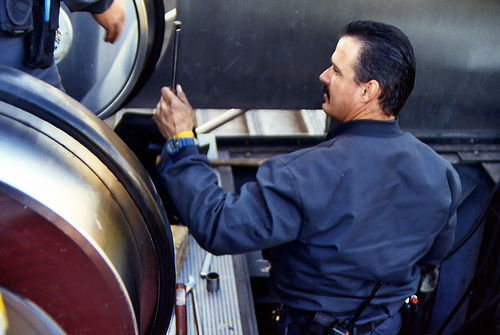
\includegraphics[width=0.775\textwidth]{1989609}
\caption{Immagine di esempio di Flickr30K (id \textit{1989609}) con le seguenti caption di riferimento: 
1) A man wearing blue coveralls is handing a tool to another person;
2) A man in a navy blue jacket holding a tool in his dirty hand;
3) A man in a work uniform passing a tool to another person;
4) Man in a blue jumpsuit attempts to repair an escalator;
5) A man with a mustache works on a broken escalator.
}
\end{figure}

\begin{figure}[ht]
\centering
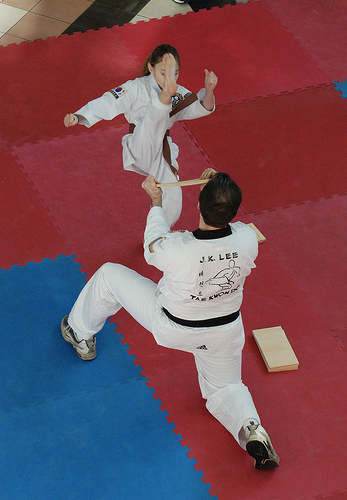
\includegraphics[width=0.5\textwidth]{101362133}
\caption{Immagine di esempio di Flickr30K (id \textit{101362133}) con le seguenti caption di riferimento: 
1) A young female student performing a downward kick to break a board held by her Karate instructor; 
2) Girl about to kick a piece of wood in half while karate instructor holds it; 
3) A girl kicking a stick that a man is holding in tae kwon do class; 
4) A girl in karate uniform breaking a stick with a front kick; 
5) A girl breaking boards by using karate. 
}
\end{figure}

\begin{figure}[H]
\centering
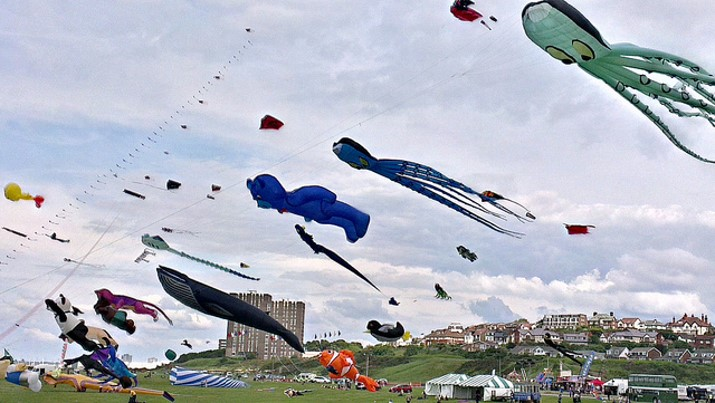
\includegraphics[width=0.8\textwidth]{000000581539}
\caption{Immagine di esempio di \acrshort{coco} (id \textit{000000581539}) con le seguenti caption di riferimento: 
1) Dozens of animal and character shaped floats flying in the air;
2) The sky is full of many colorful flying kites;
3) A bunch of colorful kites flying in the sky;
4) A large number of different kites in the air;
5) A sky filled with kites of every color next to a lush green hillside.
}
\end{figure}


\section{Metriche di valutazione}\label{metriche}
%Le valutazioni umane della traduzione automatica valutano molti aspetti della traduzione, tra cui l'adeguatezza, la fedeltà e la fluidità della traduzione. La maggior parte di questi approcci sono costosi e possono richiedere settimane o mesi per essere completati. 
%Quindi bisogna usare valutazioni automatiche che siano poco costose, veloci, indipendente dalla lingua e altamente correlata alla valutazione umana. Per giudicare la qualità di una traduzione automatica, si misura la sua vicinanza a una o più traduzioni umane di riferimento secondo una metrica numerica.
%Di seguito verranno riportate le metriche di valutazione più utilizzate nello stato dell'arte per valutare i modelli di Image Captioning.

\subsection{BLEU}
\acrshort{bleu} (\acrlong{bleu}) \cite{papineni2002bleu} è una metrica che valuta la qualità della traduzione di un testo e si basa sulla seguente idea: Più una traduzione automatica è vicina a una traduzione umana professionale, meglio è. 
Questa metrica confronta gli n-grammi della frase candidata con gli n-grammi delle traduzioni di riferimento e conta il numero di corrispondenze (le quali sono indipendenti dalla posizione), una traduzione candidata è buona se ne ha tante.
Questo concetto è modellato tramite la precisione che consiste nel conteggio del numero di parole della traduzione candidata che ricorrono in una qualsiasi traduzione di riferimento e il risultato viene diviso per il numero totale di parole nella traduzione candidata.
Sfortunatamente la precisione precedentemente definita non è sufficiente perché si potrebbero avere descrizioni improbabili con punteggi alti, quindi una parola di riferimento deve essere considerata esaurita dopo che è stata identificata una parola candidata corrispondente. L'osservazione precedentemente indicata viene formalizzata tramite la precisione modificata degli n-grammi (Modified n-gram precision), la quale viene calcolata effettuando il conteggio del numero massimo di volte con cui un n-gramma ricorre in ogni singola traduzione di riferimento. Successivamente, si taglia (clip) il conteggio totale di ogni n-gramma per il suo conteggio massimo di riferimento, si sommano i conteggi ottenuti e si divide per il numero totale di n-grammi candidati ottenendo un punteggio $p_n$. La precisione è calcolata separatamente per ogni ordine degli n-grammi, poi le precisioni calcolate sono combinate tramite una media geometrica. Questa misura cattura due aspetti della traduzione: adeguatezza e fluidità. Una traduzione che usa le stesse parole (unigrammi) dei riferimenti tende a soddisfare l'adeguatezza, mentre le corrispondenze di n-grammi più lunghe sono responsabili della fluidità.
La precisione modificata degli n-grammi decade in modo esponenziale con n e \acrshort{bleu} risolve questo problema usando il logaritmo medio con pesi uniformi, che equivale a usare la media geometrica delle precisioni modificate degli n-grammi.
La precisione modificata degli n-grammi penalizza le parole spurie nel candidato che non appaiono in nessuna delle traduzioni di riferimento, quindi il punteggio è penalizzato se una parola ricorre più frequentemente in una traduzione candidata rispetto al suo numero massimo di riferimento. Questo premia l'uso di una parola tutte le volte che è giustificato e penalizza l'uso di una parola più volte di quanto non ricorra in nessuno dei riferimenti. 
Inoltre, questa metrica riesce a penalizzare le traduzioni candidate più lunghe dei loro riferimenti e per gestire le frasi troppo brevi viene utilizzato un fattore moltiplicativo di penalità per la brevità.
Infine, il punteggio \acrshort{bleu} varia da 0 a 1 e per ottenere il valore massimo di 1 la didascalia deve essere identica a una traduzione di riferimento.
\begin{equation*}
BLEU = BP \cdot exp(\sum_{n=1}^N w_n \cdot log(p_n))
\end{equation*}
dove $p_n = \frac{\sum_{C \in \{Candidates\}} \sum_{n-gram \in C} Count_{clip} (n-gram)} {\sum_{C' \in \{Candidates\}} \sum_{n-gram' \in C'} Count_{clip} (n-gram')}$ è la precisione modificata degli n-grammi, Candidates indica le frasi candidate, $w_n = \frac{1}{N}$ sono i pesi uniformi e N indica la tipologia di N-grammi considerati (per esempio, \acrshort{bleu}@4 usa N pari a 4 e considera n-grammi composti da 1 a 4 elementi). Mentre $Count_{clip} = min(Count, MaxRefCount)$ indica il taglio tra il conteggio totale di ogni n-gramma con il suo conteggio massimo di riferimento.
BP è la penalità che regola la brevità e vale 1 se c > r altrimenti $e^{1-r/c}$ se  $c \leq r$, dove c è la lunghezza della didascalia candidata e r è la lunghezza effettiva del corpus di riferimento.
%(insieme delle caption)

\subsection{METEOR}
\acrshort{meteor} (\acrlong{meteor}) \cite{banerjee2005meteor} è una metrica per la valutazione della traduzione che si basa sulla corrispondenza di unigrammi tra la traduzione prodotta dalla macchina e le traduzioni di riferimento prodotte dall'uomo. 
Data una coppia di didascalie da confrontare questa metrica crea un allineamento tra le due stringhe. Quest'ultimo è definito come una mappatura tra gli unigrammi tale che ogni unigramma in ogni stringa corrisponda a zero o a un unigramma nell'altra stringa e a nessun unigramma nella stessa stringa. Così in un dato allineamento, un singolo unigramma in una stringa non può corrispondere a più di un unigramma nell'altra stringa. Questo allineamento è prodotto in modo incrementale attraverso una serie di stadi, i quali prevedono due fasi distinte:
\begin{enumerate}
\item Vengono usati dei moduli esterni diversi che elencano tutte le possibili mappature di unigrammi tra le due stringhe in base a diversi criteri. I moduli utilizzati sono: "exact" mappa due unigrammi se sono esattamente uguali; "porter stem" mappa due unigrammi se sono gli stessi dopo che sono stati stemmatizzati usando lo stemmer Porter; "WN synonymy" mappa due unigrammi se sono sinonimi l'uno dell'altro.
Per impostazione predefinita, il primo stadio utilizza il modulo di mappatura "exact", il secondo il modulo "porter stem" e il terzo il modulo "WN synonymy".
\item Viene selezionato il più grande sottoinsieme delle mappature generate tramite la prima fase, affinché l'insieme risultante costituisca un allineamento dove ogni unigramma corrisponde ad al massimo un unigramma nell'altra stringa. Se più di un sottoinsieme costituisce un allineamento, e ha anche la stessa cardinalità dell'insieme più grande, \acrshort{meteor} seleziona l'insieme che ha il minor numero di incroci di mappature di unigrammi. Formalmente, due mappature di unigrammi ($t_i$, $r_j$) e ($t_k$, $r_l$) (dove $t_i$ e $t_k$ sono unigrammi nella traduzione del sistema mappati rispettivamente agli unigrammi $r_j$ e $r_l$ nella traduzione di riferimento) si dicono incrociate se e solo se la seguente formula valuta un numero negativo:
\begin{equation*}
(pos(t_i) - pos(t_k)) \cdot (pos(r_j)-pos(r_l))
\end{equation*}
dove pos($t_x$) indica la posizione numerica dell'unigramma $t_x$ nella stringa del sistema, mentre pos($r_y$) indica la posizione numerica dell'unigramma $r_y$ nella stringa di riferimento. 
\end{enumerate}
Ogni stadio mappa solo gli unigrammi che non sono stati mappati a nessun unigramma in nessuna delle fasi precedenti. Quindi l'ordine in cui gli stadi vengono eseguiti impone diverse priorità sui moduli di mappatura impiegati dai diversi stadi. La metrica \acrshort{meteor} mappa prima due unigrammi in base alla loro forma superficiale, ed esegue lo stemming solo se le forme superficiali non corrispondono (o se la mappatura basata sulle forme superficiali risulta troppo "costosa" in termini di numero totale di incroci). Per impostazione predefinita, il primo stadio utilizza il modulo di mappatura "esatto", il secondo il modulo "porter stem" e il terzo il modulo "WN synonymy".
Una volta che tutti gli stadi sono terminati ed è stato generato un allineamento finale tra la didascalia del sistema e la didascalia di riferimento, il punteggio \acrshort{meteor} per questa coppia di traduzioni è calcolato così:
\begin{equation*}
METEOR = Fmean \cdot (1 - Penalty)
\end{equation*}
Dove $Fmean = \frac{10\cdot PR}{R+9\cdot P}$ è la media armonica tra la precision P e la recall R, viene assegnata più importanza alla recall.
$P = \frac{m}{w_t}$ è calcolata come il rapporto tra il numero di unigrammi nella traduzione del sistema che sono mappati (m) e il numero totale di unigrammi nella traduzione del sistema ($w_t$). Mentre $R = \frac{m}{w_r}$ è calcolato come il rapporto tra il numero di unigrammi nella traduzione del sistema che sono mappati (m) e il numero totale di unigrammi nella traduzione di riferimento ($w_r$).
Infine, $Penalty = 0.5 \cdot (\frac{\#chuncks}{\#unigrams\_matched})^3$ è una penalità che gestisce le corrispondenze lunghe, la quale considera tutti gli unigrammi nella traduzione del sistema che sono mappati a unigrammi nella traduzione di riferimento. Gli unigrammi mappati sono raggruppati nel minor numero possibile di chunks affinché essi siano in posizioni adiacenti nella traduzione del sistema, e siano anche mappati a unigrammi che sono in posizioni adiacenti nella traduzione di riferimento. 


Riassumendo questa metrica abbina gli unigrammi in base alle loro forme superficiali, alle forme stemmate e ai significati. Quindi, l'abbinamento implementato supporta non solo la corrispondenza tra parole che sono identiche nelle due stringhe confrontate, ma può anche abbinare parole che sono semplici varianti morfologiche l'una dell'altra (cioè che hanno la stessa radice), e parole che sono sinonimi l'una dell'altra. Una volta trovate tutte le corrispondenze generalizzate di unigrammi tra le due stringhe, viene usata la metrica \acrshort{meteor} per assegnare un punteggio a questa corrispondenza sfruttando una combinazione di unigram-precision, unigram-recall e una misura di frammentazione. Quest'ultima è progettata per catturare direttamente quanto le parole abbinate nella traduzione automatica siano ben ordinate in relazione al riferimento.
Se è disponibile più di una caption di riferimento, la didascalia predetta viene valutata rispetto a ciascun riferimento in modo indipendente e viene riportato il punteggio migliore.
Il valore della metrica varia tra -1,0 (correlazione completamente negativa) e +1,0 (correlazione completamente positiva). 

\subsection{CIDEr}\label{cider}
\acrshort{cider} (\acrlong{cider}) \cite{vedantam2015cider} è una metrica nata appositamente per la valutazione delle performance dei modelli di Image Captioning, misura la somiglianza di una frase generata con un insieme di frasi di verità scritte da esseri umani ed è fortemente correlata al giudizio umano. La somiglianza delle frasi permette di catturare implicitamente le nozioni di grammaticalità, salienza, importanza e accuratezza (precision e recall).
Data una frase candidata e un insieme di descrizioni di immagini Si = {$si_1$, . . . , $si_m$} di riferimento. Tutte le parole nelle frasi (sia quelle candidate che quelle di riferimento) vengono mappate alle loro forme radici e ogni frase viene rappresentata dall'insieme di n-grammi presenti in essa.
Successivamente viene usata la tecnica \acrfull{tfidf} per effettuare una rappresentazione vettoriale di ogni n-gramma $w_k$. Questa tecnica codifica quanto spesso gli n-grammi nella frase candidata sono presenti nelle frasi di riferimento, quanto gli n-grammi non presenti nelle frasi di riferimento non dovrebbero essere presenti nella frase candidata e quanto gli n-grammi che ricorrono comunemente in tutte le frasi del set di dati dovrebbe avere un peso inferiore, poiché probabilmente sono meno informativi. 
Il numero di volte che un n-gramma $w_k$ ricorre in una frase di riferimento $s_{ij}$ è indicato con $h_k(s_{ij})$ o $h_k(c_i)$ per la frase candidata $c_i$.
La rappresentazione \acrshort{tfidf} $g_k(s_{ij})$ per ogni n-gramma $w_k$ della frase $s_{ij}$ è calcolato tramite:
\begin{equation*}
g_k(s_{ij}) = \frac{h_k(s_{ij})}{\sum_{w_l\in \Omega} h_l(s_{ij})} \cdot log(\frac{|I|}{\sum_{I_p \in I} min(1, \sum_q h_k (s_{pq}))})
\end{equation*}
dove $\Omega$ è il vocabolario di tutti gli n-grammi e I è l'insieme delle immagini.
Infine, il punteggio \acrshort{cider}$_n$ per n-grammi di lunghezza n è calcolato usando la media della similarità del coseno tra la frase candidata e le frasi di riferimento, la formula è la seguente:
\begin{equation*}
CIDEr_n(c_i, S_i) = \frac{1}{m} \sum_j \frac{g_n(c_i) \cdot g_n(s_{ij})} {||g_n(c_i)|| \cdot ||g_n(s_{ij}) ||}
\end{equation*}
dove $g_n(c_i)$ è il vettore che contiene la rappresentazione \acrshort{tfidf} di $c_i$, mentre $g_n(s_{ij})$ contiene quella di $s_{ij}$.
Vengono usati n-grammi più lunghi per catturare proprietà grammaticali e una semantica più ricca (empiricamente il valore migliore è N=4), i quali sono combinati tramite:
\begin{equation*}
CIDEr(c_i, S_i) = \sum^N_{n=1} \frac{1}{N} \cdot CIDEr_n(c_i, S_i)
\end{equation*}
\subsection{SPICE}
\acrshort{spice} (\acrlong{spice}) \cite{anderson2016spice} è una metrica nata per la valutazione delle performance dei modelli di Image Captioning e misura la qualità delle didascalie generate analizzando il loro contenuto semantico.
%Questa metrica risolve i limiti delle metriche di valutazione automatica basate sugli n-grammi, la sovrapposizione di n-grammi non è né necessaria né sufficiente perché due frasi trasmettano lo stesso significato.
Le didascalie candidate C e quelle di riferimento S vengono trasformate in una rappresentazione semantica basata sugli scene graph. Questa tipologia di grafo codifica esplicitamente gli oggetti, gli attributi e le relazioni che si trovano nelle didascalie delle immagini, astraendo la maggior parte delle idiosincrasie lessicali e sintattiche del linguaggio naturale nel processo.
Viene costruito un grafo per la didascalia candidata, indicato con G(C), e un grafo per le didascalie di riferimento S, indicato con G(S); quest'ultimo è ottenuto come l'unione dei grafi di scena G($s_i$) $\forall(s_i \in S)$ combinando i nodi di oggetti sinonimi.
\begin{equation*}
G(C) = (O(C), E(C), K(C))
\end{equation*}
I grafi hanno come nodi O($\cdot$) gli oggetti menzionati nella didascalia e come archi E($\cdot$) le relazioni tra gli oggetti, inoltre i nodi prevedono degli attributi K($\cdot$).
La costruzione del grafo prevede due fasi:
\begin{enumerate}
\item Estrazione di alberi di dipendenza tramite lo Stanford Scene Graph Parser, il quale identifica le dipendenze sintattiche tra le parole delle didascalie;
\item Conversione degli alberi di dipendenza in scene graph utilizzando un sistema a regole;
\end{enumerate}
Per valutare la somiglianza dei grafi candidati e di riferimento, le relazioni semantiche nel grafo sono trattate come una congiunzione di proposizioni logiche, o tuple. La seguente funzione T restituisce tuple logiche da uno scene graph:
\begin{equation*}
T(G(C))  \stackrel{\Delta}{=} O(C) \cup E(C) \cup K(C)
\end{equation*}
Ogni tupla contiene da uno a tre elementi, i quali rappresentano rispettivamente oggetti, attributi e relazioni.
La metrica \acrshort{spice} assume un valore tra 0 e 1, la formula è la seguente:
\begin{equation*}
SPICE(C,S) = F_1(C,S) = \frac{2 \cdot P(C,S) \cdot R(C,S)}{P(C,S) + R(C,S)}
\end{equation*}
Dove $P(C,S) = \frac{|T(G(C)) \bigotimes T(G(S))|}{|T(G(C))|}$ è la precision, mentre $R(C,S) = \frac{|T(G(C)) \bigotimes T(G(S))|}{|T(G(S))|}$ è la recall e $\bigotimes$ è l'operatore di corrispondenza binaria che restituisce le tuple corrispondenti tra due scene graph (le tuple sono considerate corrispondenti se la loro forma radice è uguale).
\acrshort{spice} misura quanto bene i generatori di didascalie recuperano gli oggetti, gli attributi e le relazioni tra loro; presuppone implicitamente che le didascalie siano ben formate.
